\thispagestyle{plain}
\section{La estructura de la materia y sus modelos}

\boxabstract{Aprendizajes esperados:}{
    \begin{itemize}
        \item Deduce información acerca de la estructura atómica
              a partir de datos experimentales sobre propiedades
              atómicas periódicas.
        \item Representa y diferencia mediante esquemas, modelos y
              simbología química, elementos y compuestos, así como
              átomos y moléculas.
        \item Explica y predice propiedades físicas de los materiales
              con base en modelos submicroscópicos sobre la
              estructura de átomos, moléculas o iones, y sus
              interacciones electrostáticas.
    \end{itemize}
}
\subsection{¿Cómo los átomos y las moléculas hacen distintas a las sustancias}

\begin{boxK}
    \begin{enumerate}
        \item Anota en la tabla dos propiedades que distinguen a las sustancias que se indican y con
              las que de seguro estás en contacto frecuentemente.
        \item Dibuja qué verías si observaras cada sustancia con un microscopio muy potente.
        \item Compara tus ideas y dibujos con los de un compañero y comenten: \\
              \textbf{¿cómo explican sus dibujos las propiedades macroscópicas de las sustancias que representaron?}
              \begin{figure}[H]
                  \centering
                  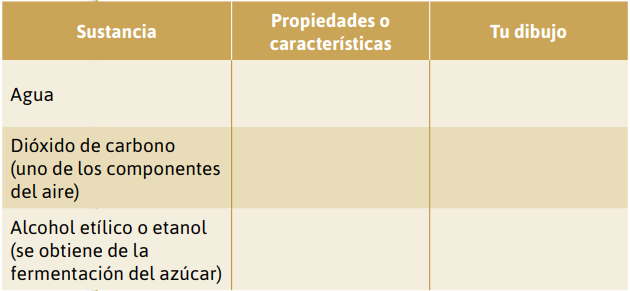
\includegraphics[width=0.7\linewidth]{tabla01.png}
                  %\captionof{table}{Modelo geométrico de la situación.}
                  \label{tab:tabla01}
              \end{figure}%
    \end{enumerate}
\end{boxK}

\subsubsection{\'Atomos y moléculas}

¿Por qué el carbón es una sustancia sólida negra y quebradiza que se quema con facilidad?
¿Por qué el azúcar es dulce y se disuelve en el agua? A lo largo de la historia, los químicos han realizado
diversos experimentos para comprender por qué cada sustancia tiene propiedades distintas.\\

Los resultados experimentales se pueden explicar mediante el modelo
cinético de partículas que estudiaste en tu curso de Ciencia y tecnología, Física, el cual supone que:

\begin{figure}[H]
    \centering
    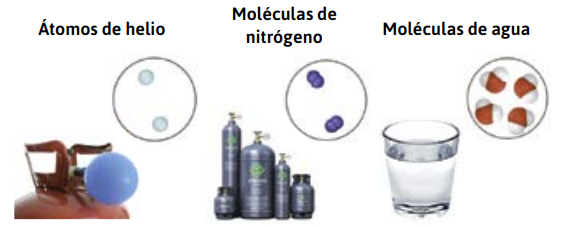
\includegraphics[width=.6\linewidth]{atomos01.png}
    \captionof{figure}{\footnotesize Representación de las partículas que constituyen diversas
        sustancias. Los átomos de distintos tipos se representan comúnmente
        como esferas de diferente color.}
    \label{fig:atomos01}
\end{figure}

%\begin{boxM}
\begin{itemize}
    \item[\checkmark] Las sustancias están constituidas por miles de millones de partículas pequeñísimas
          en constante movimiento e interacción;
    \item[\checkmark] Las partículas de una sustancia son idénticas entre sí y tienen una composición y
          estructura determinadas, que son diferentes a las de otras sustancias;
    \item[\checkmark] Las partículas de cada sustancia por lo general están constituidas por unidades más
          pequeñas llamadas \textbf{átomos}, unidos unos a otros por fuerzas de atracción llamadas \textbf{enlaces químicos}.
\end{itemize}
%\end{boxM}

Algunas sustancias elementales, como el helio y el argón, están constituidas por partículas de un solo átomo; sin embargo, las
partículas de muchas otras sustancias se forman por la unión, mediante enlaces químicos, de dos o más átomos; a estas partículas
se les llama \textbf{moléculas} (figura \ref{fig:atomos01}).

Por ejemplo, el gas nitrógeno del aire está constituido por moléculas de dos átomos
idénticos, mientras que las moléculas de agua están formadas por dos átomos de
hidrógeno unidos a un átomo de oxígeno (átomos de diferente tipo).
Las diferencias en las propiedades de las sustancias se deben a los distintos tipos
y números de átomos de las partículas que las constituyen y a la forma en que los
átomos se enlazan unos a otros.\\

\begin{boxK}
    \begin{wrapfigure}{r}{0.25\textwidth}
        \centering
        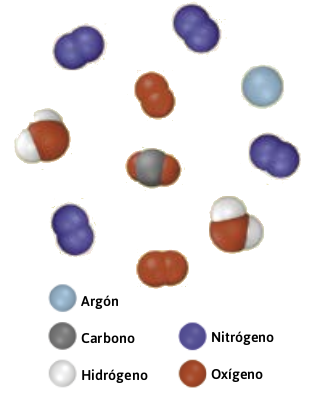
\includegraphics[width=0.25\textwidth]{atomos02.png}
        \label{fig:atomos02}
    \end{wrapfigure}
    Analiza y reflexiona:\\
    \begin{enumerate}
        \item Observa la representación de las partículas que
              forman algunas sustancias del aire que respiras.
              El código de color que por lo común se utiliza
              para representar átomos de distintos tipos es el
              que se muestra.
        \item Determina cuántas sustancias distintas se representan.
        \item Determina qué sustancias están constituidas por átomos independientes y cuáles por moléculas.
        \item Describe las semejanzas y diferencias de las moléculas que identificaste: considera tipo y cantidad de átomos.
        \item Compara tus respuestas con las de tus compañeros y valídenlas.
    \end{enumerate}%
    % \end{minipage}
\end{boxK}

\subsubsection{Sustancias elementales y compuestos químicos a nivel nanoscópico}

Como estudiaste en la unidad anterior, existen sustancias elementales que no se pueden descomponer
en otras más simples mediante procesos químicos. El nitrógeno y el oxígeno del aire son
ejemplos de sustancias elementales. Por otro lado, los compuestos
químicos sí se descomponen en sustancias elementales a partir
de métodos químicos. Algunos ejemplos son el agua, que puede
descomponerse en hidrógeno y oxígeno, y el dióxido de carbono
que exhalamos, que se descompone en oxígeno y carbono.\\

\begin{wrapfigure}{r}{0.4\textwidth}
    \centering
    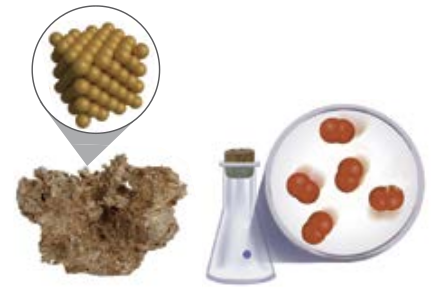
\includegraphics[width=0.4\textwidth]{atomos03.png}
    \captionof{figure}{\footnotesize El cobre y el oxígeno son sustancias
        elementales constituidas por átomos del mismo
        tipo.}
    \label{fig:atomos03}
\end{wrapfigure}

La idea de que las sustancias están constituidas por diferentes
tipos de átomos permite explicar la diferencia entre sustancias elementales y
compuestos químicos. Las elementales no pueden descomponerse en sustancias más simples porque están constituidas
por partículas con el mismo tipo de átomo.\\

Por ejemplo, el cobre con el que se fabrican cables, está conformado por átomos idénticos ordenados uno junto a otro,
mientras que el oxígeno que respiramos tiene moléculas con dos átomos de oxígeno cada una (figura
\ref{fig:atomos03}). Por su parte, los compuestos químicos se pueden descomponer en sustancias elementales
porque están constituidos por partículas con átomos de distintos tipos. Los átomos que conforman las moléculas de agua, por ejemplo, se pueden separar
y reorganizarse para formar las sustancias elementales hidrógeno y oxígeno (figura \ref{fig:atomos04}).\\

\begin{figure}[H]
    \centering
    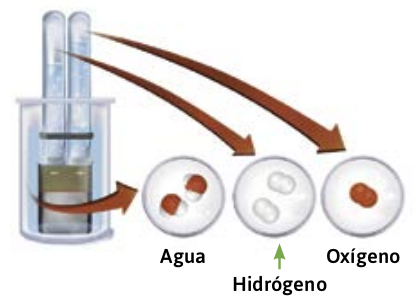
\includegraphics[width=0.5\textwidth]{atomos04.png}
    \captionof{figure}{El agua se logra descomponer en
        hidrógeno y oxígeno mediante el paso de
        corriente eléctrica.}
    \label{fig:atomos04}
\end{figure}

\subsubsection{Tipos de \'atomos}

La separación e identificación de las diferentes sustancias elementales que
hay en la naturaleza ha permitido determinar los distintos tipos de átomos
que existen. En la actualidad se han identificado más de 100 átomos
distintos, y las partículas de todas las sustancias conocidas, naturales o sintéticas,
son resultado de la combinación de esos átomos
(figura \ref{fig:atomos07}). Cada tipo de átomo corresponde con un elemento
químico y se le asigna un símbolo particular.

Por ejemplo, los
átomos de oxígeno se representan con el símbolo \emph{O}, mientras que
los átomos de hidrógeno, con el símbolo \emph{H}. Los símbolos que representan
cada tipo de átomo no siempre corresponden con las primeras letras
de su nombre en español, porque algunos se derivan del nombre de las sustancias
en otros idiomas, como el latín.\\

\begin{minipage}{\textwidth}
    \begin{boxK}
        Observa y representa:

        \begin{enumerate}
            \item Distingue similitudes y diferencias en las representaciones de las siguientes
                  moléculas de distintas sustancias.

                  \begin{figure}[H]
                      \centering
                      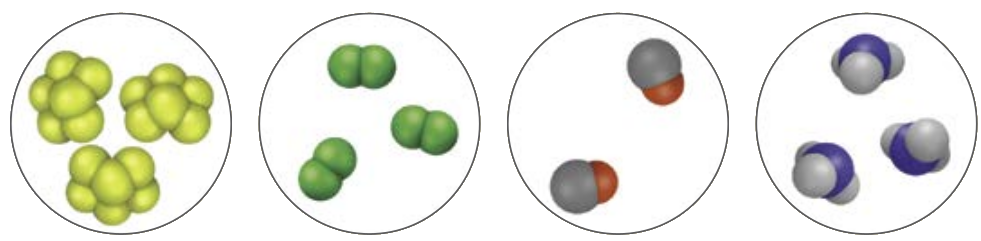
\includegraphics[width=.6\textwidth]{atomos05.png}
                  \end{figure}

            \item Identifica cuáles representan sustancias elementales y cuáles compuestos químicos. Justifica tus decisiones.
            \item Usa las representaciones anteriores para representar una mezcla constituida por
                  partículas de una sustancia elemental y partículas de un compuesto químico.
            \item Compara y contrasta tus dibujos con los de tus compañeros.
        \end{enumerate}
    \end{boxK}
\end{minipage}
\vspace{0.5cm}

\begin{wrapfigure}{l}{0.4\textwidth}
    \centering
    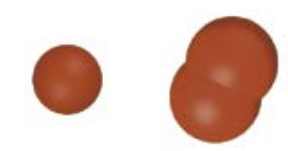
\includegraphics[width=0.3\textwidth]{atomos07.png}
    \captionof{figure}{\footnotesize Las propiedades y estructura de estas sustancias son diferentes aunque tengan el mismo tipo de átomo.}
    \label{fig:atomos07}
\end{wrapfigure}

Para el sodio, por ejemplo, el símbolo es Na porque proviene de su nombre en latín, natrium, que significa raro.
Los diferentes átomos o elementos químicos conocidos se listan en la
tabla periódica de los elementos (figura \ref{tab:periodic_table}, p. \pageref{tab:periodic_table}). Los que se localizan en la misma hilera pertenecen
al mismo periodo. Los átomos o elementos incluidos en la tabla periódica tienen el mismo
nombre que la sustancia elemental en la que están presentes, pero las propiedades de esos átomos no son
las mismas que las de las sustancias elementales.\\

\begin{wrapfigure}{l}{0.45\textwidth}
    \centering
    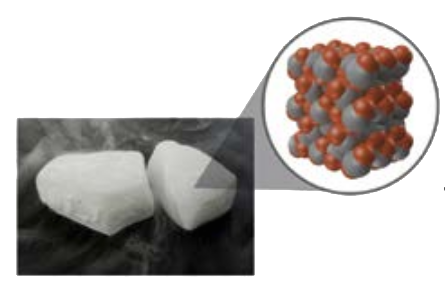
\includegraphics[width=0.45\textwidth]{atomos06.png}
    \captionof{figure}{\footnotesize El hielo seco (dióxido de
        carbono sólido) es un compuesto químico constituido por los elementos carbono y oxígeno.}
    \label{fig:atomos06}
\end{wrapfigure}

Por ejemplo, el oxígeno gaseoso presente en el aire que respiramos
está constituido por moléculas de dos átomos de oxígeno cada una. Los seres
humanos inhalamos sin problema las moléculas de oxígeno contenidas en
el aire, pero si en lugar de moléculas respiráramos átomos de oxígeno separados, podríamos morir (figura \ref{fig:atomos06}).\\

Las propiedades de las sustancias elementales no sólo dependen del tipo de átomos que las componen, sino también
de cómo estos se enlazan en las partículas que los constituyen.
Por ejemplo, el grafito que contiene la punta de los lápices
es una sustancia elemental suave y quebradiza hecha de
átomos de carbono (C), mientras que el diamante, que es duro
y resistente, también es una sustancia elemental formada por
átomos de carbono (figura \ref{fig:atomos07}).\\

\begin{boxK}
    Analiza y genera hipótesis
    \begin{enumerate}
        \item Discute con tus compañeros sobre cómo es posible que
              dos sustancias con propiedades tan distintas como el
              diamante y el grafito estén constituidas por el mismo
              tipo de átomos (carbono, C).
    \end{enumerate}
\end{boxK}

\subsubsection{Simbología química}

Los químicos han desarrollado distintas maneras de representar la composición y
estructura de las sustancias elementales y de los compuestos químicos de nuestro
entorno (nivel macroscópico) mediante dibujos que representan los átomos y moléculas presentes en el material.
Cuando describimos el comportamiento de las sustancias
y los materiales representando los átomos y moléculas que los forman se dice que
hacemos una descripción a nivel nanoscópico.
En estas representaciones usamos fórmulas químicas que se hacen a partir de los
símbolos de los átomos o elementos químicos. Si las moléculas poseen átomos iguales,
se usan subíndices para indicar el número de átomos de cada tipo. Por ejemplo, la
fórmula química de las moléculas del oxígeno que respiramos es O$_2$ , lo cual indica que
cada una está constituida por dos átomos de oxígeno. La fórmula química de las moléculas de dióxido de carbono es CO$_2$;
esto indica que están formadas por un átomo de
carbono y dos de oxígeno. Si se necesita representar una sustancia con gran cantidad
de partículas en estado sólido, líquido o gaseoso, los símbolos (s), (l) y (g) se colocan a
la derecha de la fórmula: CO$_2$ (s) representa una muestra de dióxido de carbono sólido
(hielo seco) y O$_2$ (g) representa una muestra de oxígeno gaseoso.\\

En esta lección has aprendido que las diferencias en las propiedades de las sustancias
se deben a la composición de las partículas que las constituyen, la cual se representa
mediante esquemas que muestran la composición atómica de las partículas o el uso
de fórmulas químicas. Para evaluar lo que has aprendido, haz la siguiente actividad.

\newpage
\begin{landscape}
    \thispagestyle{plain}
    %\newgeometry{left=-50mm,top=-30mm,bottom=-30mm,right=-30mm}
    \begin{figure}[H]
        \TablaPeriodica[0.48]
        \captionof{table}{Tabla Peri\'odica de los Elementos.}
        \label{tab:periodic_table}
    \end{figure}
    %\restoregeometry
\end{landscape}

\newpage
\begin{boxK}
    \begin{enumerate}
        \item Completa la información de la tabla.
        \item Compara y contrasta la composición de las partículas que constituyen las distintas sustancias.
        \item Compara estas representaciones con las que hiciste al inicio de esta lección
              (p. 100): ¿cómo cambiaron? ¿Qué ventajas y desventajas tiene una representación respecto a la otra?
              \begin{figure}[H]
                  \centering
                  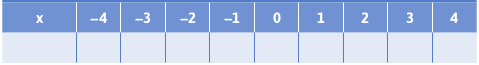
\includegraphics[width=.8\textwidth]{tabla02.png}
              \end{figure}

    \end{enumerate}
\end{boxK}

\newpage
\subsection{¿Qué hace a un átomo diferente de otro?}

\begin{boxK}
    \begin{enumerate}
        \item Explora las propiedades eléctricas de distintos materiales; por ejemplo, infla un globo
              (también puedes utilizar un vaso de plástico) y frótalo sobre tu cabello. Enseguida,
              acerca el globo a distintos materiales, como pequeños trozos de papel,
              una bolsa de plástico, un vaso de unicel, una lata de aluminio o un
              chorro fino de agua y de otras sustancias.
        \item Observa qué pasa en cada caso.
        \item Discute con tus compañeros por qué piensas que el material del que
              está hecho el globo interacciona de diferentes maneras con los otros
              materiales. Recuerda lo que aprendiste en tu curso de Ciencia y tecnología,
              Física sobre interacciones eléctricas.
        \item Discutan qué sucede a nivel nanoscópico con los átomos y las moléculas
              de las que están hechos estos materiales cuando los frotan.
    \end{enumerate}

\end{boxK}

\subsubsection{Componentes atómicos}

Un gran número de experimentos, como el propuesto en la actividad de inicio, sugieren
que la materia tiene propiedades eléctricas. En tu curso de Física aprendiste que
científicos como Thomson y Rutherford, a partir de distintos experimentos, detectaron
partículas (llamadas subatómicas) con cargas positivas y negativas en los átomos
y moléculas que constituyen las sustancias químicas. Con esta información propusieron
modelos para describir la estructura de los átomos, como el que se representa en
la figura \ref{fig:atomos08}.\\

\begin{figure}[H]
    \centering
    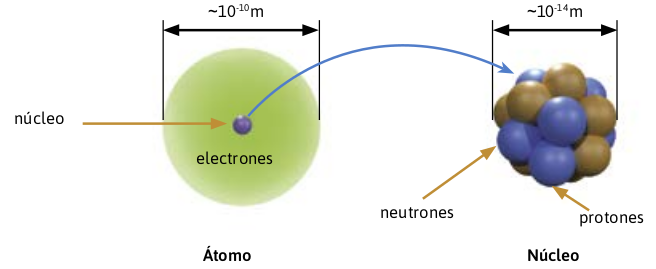
\includegraphics[width=0.7\linewidth]{atomos08.png}
    \captionof{figure}{\footnotesize Representación de la estructura de un átomo.}
    \label{fig:atomos08}
\end{figure}%

De acuerdo con este modelo atómico, cada átomo está constituido por partículas
con carga positiva, llamadas \textbf{protones}, concentradas en un núcleo muy pequeño, y por
partículas con carga negativa, denominadas \textbf{electrones}, que se mueven a su alrededor.
El núcleo de los átomos contiene otro tipo de partículas sin carga eléctrica (partículas
neutras) conocidas como \textbf{neutrones}. Los electrones son partículas muy pequeñas y
ligeras (poca masa), mientras que los protones y neutrones son de mayor tamaño y
poseen una masa 2 000 veces mayor que la del electrón. Cada átomo tiene el mismo
número de protones que de electrones y, por tanto, es eléctricamente neutro. Los electrones
se mantienen en movimiento alrededor del núcleo por la atracción entre cargas
eléctricas negativas y positivas.


\begin{boxK}
    Compara y analiza:\\
    \begin{enumerate}
        \item Lee y usa la información que se muestra en la imagen para determinar cuántas
              veces es más pequeño un átomo comparado con los objetos y organismos. Si es
              necesario, investiga el valor de las unidades de medida representadas.
              \begin{boxF}
                  Los átomos son partículas muy pequeñas. En el diámetro de uno de tus cabellos se podrían
                  acomodar en hilera unos 500 000 átomos de carbono. Si un cabello se pudiera agrandar
                  hasta alcanzar el diámetro de nuestro planeta, un átomo del cabello tendría el tamaño de
                  una cancha de basquetbol.
              \end{boxF}

              \begin{figure}[H]
                  \centering
                  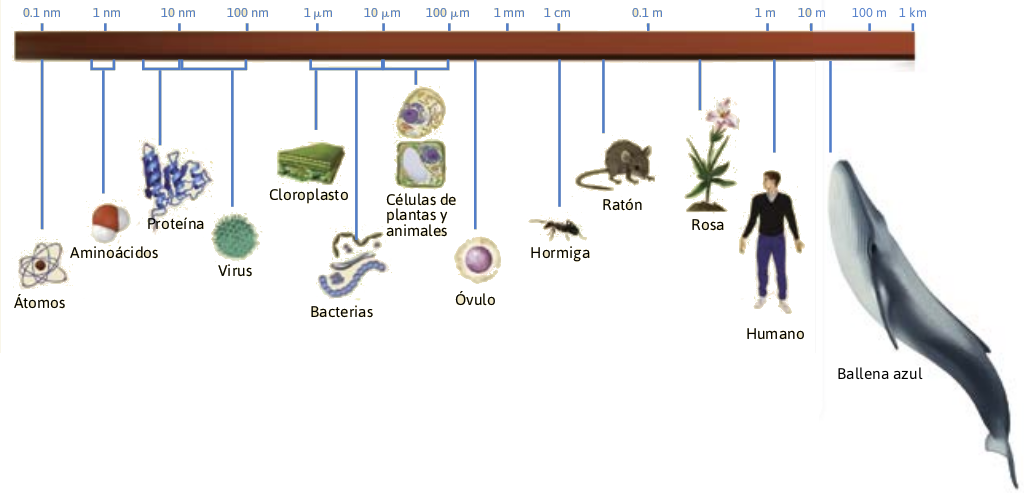
\includegraphics[width=.8\textwidth]{escala.png}
              \end{figure}


        \item Compara tus respuestas y métodos con los de otros compañeros y valídenlos.
    \end{enumerate}
\end{boxK}
\newpage

\subsubsection{Identidad atómica}

\begin{wrapfigure}{r}{0.35\textwidth}
    \centering
    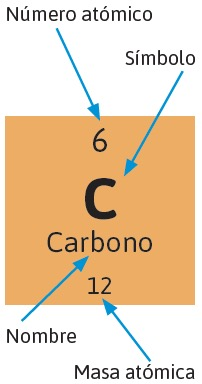
\includegraphics[width=0.45\linewidth]{eolementoCarbono.jpg}
    \captionof{figure}{\footnotesize Es importante reconocer cómo se presenta en la tabla periódica la información de cada átomo.}
    \label{fig:eolementoCarbono}
\end{wrapfigure}%

La identidad de cada átomo la determina su número de protones. Este dato se conoce como \textbf{número atómico} y
se representa con la letra Z. Por ejemplo, el átomo de hidrógeno (H) tiene en su núcleo un solo protón;
por tanto, su número atómico es Z = 1; el átomo de carbono (C) tiene seis protones y su número atómico
Z = 6. Como cada átomo es neutro, posee el mismo número de protones que de electrones; entonces, el número
atómico también indica cuántos electrones hay en cada átomo; así, el oxígeno (O) con Z = 8 está constituido
por 8 protones en el núcleo y 8 electrones que se mueven a su alrededor. El número atómico, Z, es la propiedad
que permite ordenar a los átomos de manera secuencial en la tabla periódica, y su valor se coloca sobre el símbolo
de cada elemento, como se ve en la figura \ref{fig:eolementoCarbono}.\\

La tabla periódica también contiene información sobre la \textbf{masa atómica relativa} de los distintos átomos y se
simboliza por las letras A$_r$ (figura \ref{fig:eolementoCarbono}). Medir la masa de un solo átomo es muy difícil,
pero es posible determinar cuántas veces la masa de un átomo es más grande en relación con otro.
Por ejemplo, de acuerdo con la tabla periódica,
A$_r$ = 12.0 para los átomos de carbono y Ar = 1.01 para los de hidrógeno. Esto indica que un solo átomo de carbono
es casi doce veces más pesado que uno de hidrógeno. Por su parte, la masa atómica relativa del magnesio (Mg)
es $A_r = 24.3$, lo cual implica que un átomo de este elemento es alrededor de 24 veces más pesado que uno de
hidrógeno, pero sólo dos veces más pesado que uno de carbono ($24.3/12 \sim 2$).\\

\begin{minipage}{\textwidth}
    \begin{boxK}
        Analiza e infiere:
        \begin{enumerate}
            \item Lee y organiza con tus compañeros un juego con base en preguntas y respuestas sobre cómo un átomo se compara
                  con otros de la tabla periódica. Utiliza los ejemplos que se presentan más abajo como guía para proponer tus preguntas.

                  \begin{boxF}
                      Es importante que te familiarices con las propiedades de los átomos que forman las sustancias de tu alrededor,
                      como el agua (H$_2$O), el azúcar (C$_{12}$H$_{22}$O$_{11}$) y el cloruro de sodio (sal común, NaCl).
                      Estos átomos suelen tener números atómicos menores a 30 (Z < 30) y se localizan en las cuatro primeras hileras de
                      la tabla periódica.
                  \end{boxF}
            \item ¿Cuántas veces es más pesado un átomo de calcio (Ca) que un átomo de oxígeno (O)?
            \item ¿Cuántos electrones hay en un átomo de hierro (Fe)?
            \item ¿Cuántos protones más tiene un átomo de cloro que uno de carbono (C)?
        \end{enumerate}
    \end{boxK}
\end{minipage}

\newpage
\subsubsection{Ejercicios}

\begin{boxK}
    Elige la(s) respuesta(s) correcta(s).
    \begin{enumerate}
        \item ¿Qué propiedad periódica de los elementos se representa con la letra $Z$?

              \begin{hoptboxes}
                  \item Densidad atómica
                  \item Tamaño atómico
                  \item Masa atómica
                  \item Número atómico
              \end{hoptboxes}

        \item ¿A qué cantidad de partículas equivale $Z$?

              \begin{hoptboxes}
                  \item Al número de neutrones.
                  \item Al número de fotones.\\
                  \item Al número de electrones.
                  \item Al número de protones.
              \end{hoptboxes}
        \item ¿Qué propiedad periódica de los elementos se representa como $A_r$?

              \begin{hoptboxes}
                  \item Densidad atómica relativa.
                  \item Tamaño atómico relativo.\\
                  \item Masa atómica relativa.
                  \item Número atómico relativo.
              \end{hoptboxes}
        \item El valor $A_r=5$ para los átomos de boro significa que:

              \begin{hoptboxes}
                  \item un sólo átomo de boro es casi 5 veces más pesado que uno de hidrógeno.\\
                  \item un sólo átomo de hidrógeno es casi 5 veces más pesado que uno de boro.\\
                  \item un sólo átomo de boro es casi 5 veces menos pesado que uno de hidrógeno.\\
                  \item un sólo átomo de hidrógeno es casi 5 veces menos pesado que uno de boro.
              \end{hoptboxes}
        \item ¿Qué valor de $Z$ tiene un átomo con 20 neutrones y un valor de $A_r=39$?

              \begin{hoptboxes}
                  \item Z = 20
                  \item Z = 19
                  \item Z = 49
                  \item Z = 39
              \end{hoptboxes}

    \end{enumerate}

\end{boxK}

\subsubsection{Iones: partículas con carga eléctrica}

\begin{figure}[H]
    \centering
    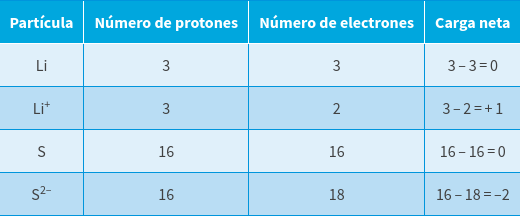
\includegraphics[width=0.7\linewidth]{tabla_de_cargas.png}
    \captionof{table}{Carga neta de algunos átomos.}
    \label{tab:tabla_de_cargas}
\end{figure}%

Los electrones de un átomo están en constante movimiento alrededor del núcleo atraídos por la carga positiva
de los protones. Como los electrones tienen carga negativa se repelen entre sí, lo que causa que algunos se
muevan cerca del núcleo atómico, mientras otros se desplazan a distancias más lejanas. Los electrones que están
más alejados del núcleo en ocasiones escapan del átomo o son atraídos por otros átomos o moléculas. Cuando esto
sucede, el átomo deja de tener el mismo número de protones y electrones y adquiere una carga eléctrica neta.
Se dice que se convierte en un \textbf{ion}.

\begin{figure}[H]
    \centering
    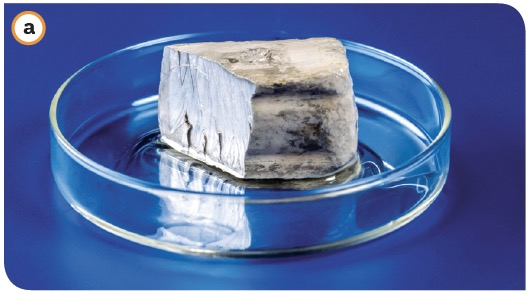
\includegraphics[width=0.40\linewidth]{sodio.jpg}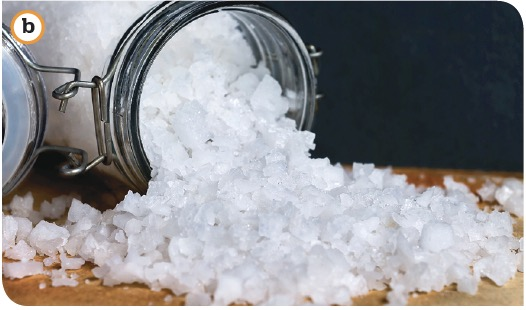
\includegraphics[width=0.40\linewidth]{sodio2.jpg}
    \captionof{figure}{\footnotesize El sodio metálico tiene propiedades muy diferentes al sodio de la sal común.
        a) Sodio metálico. b) Sal común contiene cationes de sodio (Na$^+$) y aniones de cloro (Cl$^-$).}
    \label{fig:sodio2}
\end{figure}%

Imagina, por ejemplo, que un átomo de litio (Li) con tres protones (Z = 3) perdiera uno de sus electrones.
Esta partícula tendría tres cargas positivas (+3), pero sólo dos cargas negativas (-2).
Su carga neta sería $+3 - 2 = +1$. Cuando esto sucede se dice que se forma un \textbf{ion positivo o catión},
y en el caso del litio este ion se representa con el símbolo Li$^+$. Un átomo también puede ganar electrones
atrayéndolos de otros átomos y así se transforma en un \textbf{ion negativo o anión}. Por ejemplo, si un átomo de
azufre (Z = 16) gana dos electrones, tendrá 16 protones y 18 electrones y su carga neta será $+16 - 18 = -2$.
Este anión se representa con el símbolo S$^{2-}$. La pérdida o ganancia de electrones no cambia la identidad de un
átomo, pero le da propiedades distintas. Los átomos de sodio (Na) en un pedazo de este metal interaccionan de
manera muy distinta con otras partículas a como lo hacen los iones Na+ presentes en compuestos químicos como
la sal común (figura \ref{sodio2}).


Muchos de los elementos químicos necesarios para la vida están presentes en todo nuestro cuerpo en forma de
iones, ya sea en los huesos, en la sangre y en el citoplasma de nuestras células.

\begin{boxK}
    Infiere y compara
    \begin{enumerate}
        \item Lee y completa la tabla con la información que se presenta.
              \begin{boxF}
                  Muchos compuestos químicos a nuestro alrededor están constituidos por átomos o moléculas con carga, es decir,
                  por aniones y cationes. Un ejemplo típico es el cloruro de sodio, simbolizado como NaCl, que está conformado por
                  cationes Na$^+$ y aniones Cl$^-$. En la siguiente tabla se listan otros compuestos \emph{iónicos} importantes.
              \end{boxF}

              \begin{figure}[H]
                  \centering
                  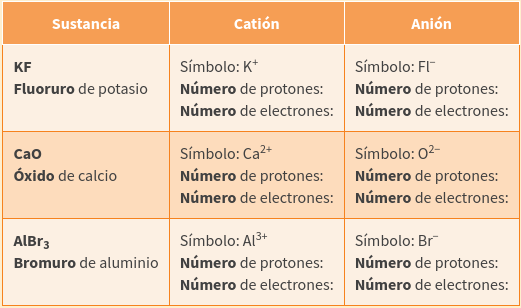
\includegraphics[width=0.6\linewidth]{tablaAnionCation.png}
                  % \captionof{table}{El sodio metálico tiene propiedades muy diferentes al sodio de la sal común.
                  %   a) Sodio metálico. b) Sal común contiene cationes de sodio (Na+) y aniones de cloro (Cl-).}
                  \label{fig:tablaAnionCation}
              \end{figure}%

              Compara tus resultados con los de algunos compañeros de clase y valídenlos en grupo y con ayuda de su maestro.
              El modelo atómico de la materia es muy útil para explicar los fenómenos que observamos cada día; en particular, permite entender las interacciones entre diversas sustancias.
    \end{enumerate}
\end{boxK}
%
\begin{boxK}
    \begin{enumerate}
        \item Recuerda los experimentos que hiciste con el globo al principio de esta lección. Discute con tus compañeros qué sucede a nivel atómico cuando el globo se frota contra distintos materiales. Apliquen los conocimientos que adquirieron en esta lección sobre estructura atómica y formación de iones.
        \item Representen a nivel nanoscópico lo que le pasa a los electrones de los átomos en la superficie del globo y del cabello cuando se frotan el uno contra el otro. A partir de su representación expliquen lo siguiente.
              \begin{enumerate}
                  \item Por qué el globo y el cabello se atraen después de frotarlos.
                  \item Por qué el globo puede atraer otros materiales después de frotarlo.
              \end{enumerate}
        \item Compartan en equipos sus resultados, corríjanlos en caso de ser necesario y valídenlos con su maestro.
    \end{enumerate}
\end{boxK}

El modelo atómico de la materia es muy útil para explicar los fenómenos que observamos cada día;
en particular, permite entender las interacciones entre diversas sustancias.

\newpage
\subsection{¿Cómo estudiamos a los átomos de manera experimental?}
\begin{boxK}
    \begin{enumerate}
        \item Consigan en equipos cajas de cartón e introduzcan en ellas uno o varios objetos: lápices, gomas,
              llaves, etcétera; cada caja puede tener diferentes objetos. Cuiden que los otros equipos no vean
              lo que colocaron en las cajas.
        \item Séllenlas con cinta adhesiva de manera que no puedan ver su contenido.
        \item Intercambien su caja con otro equipo y sin abrirlas traten de descubrir qué objetos contienen.
        \item Después hagan lo que se indica.
              \begin{enumerate}
                  \item Reflexionen en grupo sobre las pruebas o los experimentos que pueden realizar para determinar
                        el contenido de las cajas.
                  \item Pongan a prueba sus ideas y traten de inferir el contenido de la caja.
              \end{enumerate}
        \item Comprueben sus respuestas abriendo las cajas. ¿Acertaron? ¿Se equivocaron? Expliquen.
    \end{enumerate}
\end{boxK}


\subsubsection{Descubriendo sin ver}

El problema al que te enfrentaste en la actividad anterior de tratar de saber qué hay en la caja sin verlo
es análogo al que se han enfrentado los científicos para descubrir la estructura de los átomos.
Para entender y explicar cómo los átomos se unen entre sí para formar las moléculas de los diferentes
tipos de sustancias se requiere explorar su estructura interna. Pero ¿cómo hacerlo si los átomos no se
pueden ver ni con el microscopio más potente? Es probable que al investigar el contenido de la caja en
la actividad inicial usaras diferentes formas de energía para determinar su contenido.
Por ejemplo, aplicaste energía mecánica para agitarla; aprovechaste la energía sonora para identificar
los sonidos de los objetos al chocar. De manera similar, los científicos se han valido de diversos desarrollos
tecnológicos que les permiten utilizar diferentes tipos de energía para explorar las propiedades de los átomos.

\begin{figure}[H]
    \centering
    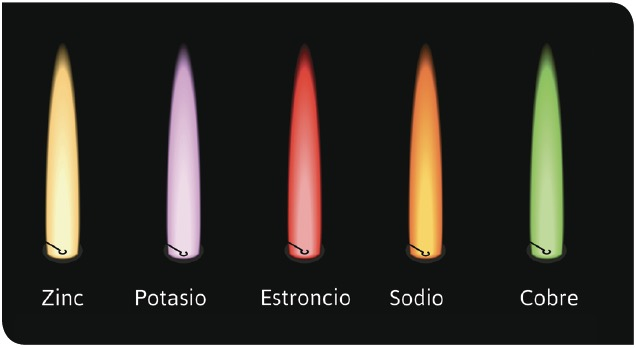
\includegraphics[width=0.5\linewidth]{flama.jpg}
    \captionof{figure}{\footnotesize Diferentes elementos químicos emiten luz de colores distintos.}
    \label{fig:flama}
\end{figure}%

Por ejemplo, en tu curso de Ciencia y tecnología, Física estudiaste que los científicos utilizaron energía
térmica para calentar muestras de diferentes elementos y analizar la luz que emitan (figura \ref{fig:flama}).
Este tipo de luz dio pistas sobre cómo se distribuyen y mueven los electrones alrededor del núcleo.



Los científicos también utilizan rayos X para medir el tamaño de los átomos.
La gráfica \ref{fig:radio_numero} muestra cómo el radio de los átomos cambia con el número atómico Z para los
primeros veinte elementos químicos de la tabla periódica.

\begin{figure}[H]
    \centering
    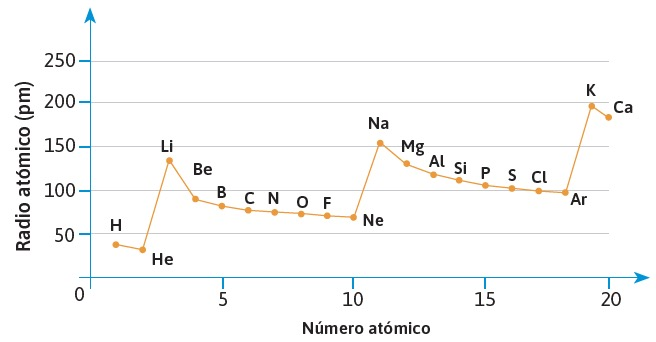
\includegraphics[width=0.8\linewidth]{radio_numero.jpg}
    \captionof{figure}{Variación del radio atómico (en picómetros) en función del número atómico
    }
    \label{fig:radio_numero}
\end{figure}%

\begin{boxF}
    Analiza e interpreta
    \begin{enumerate}
        \item Revisen en equipos los resultados experimentales que se presentan en la gráfica \ref{fig:radio_numero} sobre la variación del radio atómico en función del número atómico, Z, y respondan.
              \begin{enumerate}
                  \item ¿Cómo cambia el radio de los átomos a medida que el número atómico se incrementa para elementos dentro de un mismo periodo (hilera) en la tabla periódica?
                  \item ¿Y cómo varía a medida que el número atómico se incrementa para elementos dentro de un mismo grupo o familia (columna)?
                  \item Utilicen los datos para justificar esta afirmación: el radio atómico es una propiedad \emph{periódica} de los elementos químicos.
                  \item Propongan una hipótesis que explique las variaciones observadas en el radio de los átomos a medida que el número atómico de los elementos se incrementa en un mismo periodo y en una misma familia de la tabla periódica.
                  \item Expongan ante el grupo sus hipótesis y validen sus argumentos.
              \end{enumerate}

    \end{enumerate}
\end{boxF}

\subsubsection{Modelo de capas}

Las investigaciones sobre la estructura de distintos tipos de átomos muestran que ciertas propiedades de estas partículas,
como el radio atómico, varían de manera periódica con el número atómico. ¿Cómo podemos explicar este comportamiento?
A lo largo de la historia se han propuesto diferentes modelos sobre la estructura de los átomos para explicar este fenómeno.
Uno de ellos se conoce como modelo de capas electrónicas, que es útil para entender la periodicidad atómica.


\begin{figure}[H]
    \centering
    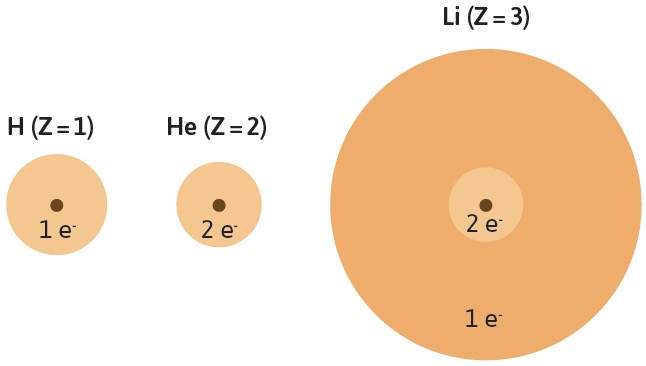
\includegraphics[width=0.4\linewidth]{capas01.jpg}
    \captionof{figure}{Distribución en capas de los electrones en los átomos de H, He y Li.}
    \label{fig:capas01}
\end{figure}

Los electrones de un átomo están en constante movimiento y no es posible determinar con precisión,
en un instante dado, su trayectoria y ubicación; sin embargo, sí se logra predecir la probabilidad de
encontrar electrones en diferentes regiones alrededor del núcleo. Para explicar los resultados
experimentales se ha propuesto que en un átomo los electrones tienden a localizarse en capas más o
menos esféricas alrededor del núcleo; sin embargo, como los electrones se repelen unos a otros, no
todos ellos están en la misma capa. Para ilustrar esta idea consideremos los tres primeros elementos
en la tabla periódica: hidrógeno (H, Z = 1), helio (He, Z = 2) y litio (Li, Z = 3).
La figura \ref{fig:capas01} ilustra cómo se distribuyen los electrones de esos átomos de acuerdo
con el modelo de capas electrónicas.



El electrón en el átomo de hidrógeno se mueve en la primera capa. En el átomo de helio, los dos electrones
también se desplazan dentro de la primera capa, pero como el átomo de helio tiene un protón más que el átomo
de hidrógeno, el núcleo atrae los dos electrones con más fuerza y por eso es un poco más pequeño que el átomo de hidrógeno.

El átomo de litio sólo tiene un electrón más que el átomo de helio, pero su tamaño es mucho mayor (figura \ref{fig:capas01}).
Para explicarlo suponemos que en el átomo de litio la repulsión entre electrones causa que el tercer electrón ocupe una capa
distinta, más alejada del núcleo. Varios electrones pueden moverse dentro de la misma capa atómica, pero hay un punto en
el que las repulsiones electrónicas obligan a los electrones adicionales a moverse en una capa más externa.
La figura \ref{fig:capas02} ilustra este fenómeno para los átomos del segundo periodo en la tabla periódica y
para el primer elemento del tercer periodo. En los átomos del segundo periodo, los dos primeros electrones se
localizan en la primera capa, y el resto se mueve en la segunda, la cual tiene la capacidad de alojar un máximo
de ocho electrones. Las interacciones entre éstos hacen que el electrón adicional en el átomo de sodio (Na, Z = 11)
se localice en una tercera capa, incrementando el tamaño de este átomo.

\begin{figure}[H]
    \centering
    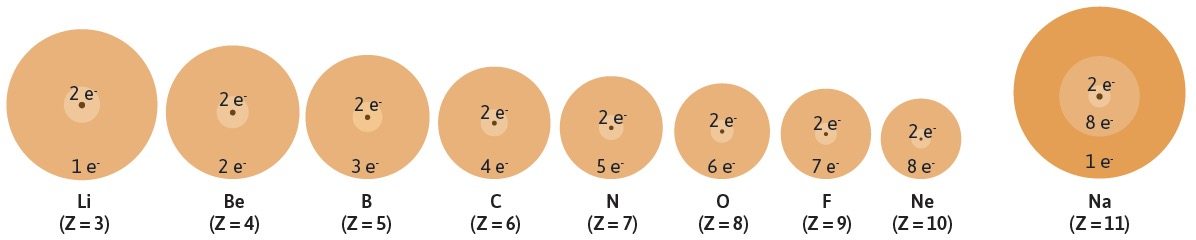
\includegraphics[width=0.9\linewidth]{capas02.jpg}
    \captionof{figure}{Distribución en capas de los electrones en átomos con Z = 3 hasta Z = 11.}
    \label{fig:capas02}
\end{figure}%

\begin{boxK}
    Analiza y explica
    \begin{enumerate}
        \item Lean y analicen en equipo cómo la energía de ionización cambia con el número atómico para elementos de un
              mismo periodo (hilera) de la tabla periódica y para elementos de un mismo grupo o familia (columna).

              \begin{boxF}
                  La gráfica \ref{fig:radio_numero} muestra la energía necesaria para arrancar un electrón de la capa más
                  externa de átomos
                  con un número atómico entre Z=1 y Z=55. Esta energía se conoce como energía de ionización de los
                  elementos, la cual entre más grande resulta más difícil para el átomo perder un electrón y convertirse en un catión.
              \end{boxF}

        \item Determina si la energía de ionización es una propiedad periódica. Justifiquen su respuesta.
        \item Expliquen, con base en el modelo atómico de capas, cómo varía la energía de ionización de los átomos a
              lo largo de un periodo y de una familia.
        \item Presenten sus respuestas y explicaciones al grupo y entre todos determinen si son lógicas y coherentes.
    \end{enumerate}
\end{boxK}
\newpage
\subsubsection{Ejercicios}
\begin{boxK}
    Relaciona la especie química con la cantidad de \textbf{protones} y \textbf{electrones de valencia}.\\

    \begin{minipage}{0.5\textwidth}
        \begin{enumerate}
            \item Magnesio (Mg)
            \item I\'on Potasio (K$^+$)
            \item Ión azufre (S2$^-$)
            \item Ión flúor (F$^-$)
            \item Ión calcio (Ca$_2^+$)
            \item Carbono (C)
            \item Ión aluminio (Al$_3^+$)
        \end{enumerate}
    \end{minipage}%
    % \vspace{2cm}
    \begin{minipage}{0.5\textwidth}
        \begin{itemize}
            \item[\rule{1cm}{0.2mm}] 20 protones y 8 electrones.
            \item[\rule{1cm}{0.2mm}] 9 protones y 8 electrones.
            \item[\rule{1cm}{0.2mm}] 16 protones y 8 electrones.
            \item[\rule{1cm}{0.2mm}] 6 protones y 4 electrones.
            \item[\rule{1cm}{0.2mm}] 13 protones y 8 electrones.
            \item[\rule{1cm}{0.2mm}] 19 protones y 8 electrones.
            \item[\rule{1cm}{0.2mm}] 12 protones y 2 electrones.
        \end{itemize}
    \end{minipage}

\end{boxK}

\begin{boxK}
    Relaciona la especie química con la cantidad de \textbf{protones} y \textbf{electrones de valencia}.\\

    \begin{minipage}{0.5\textwidth}
        \begin{enumerate}
            \item Ión oxígeno (O$_2^-$)
            \item Nitrógeno (N)
            \item Silicio (Si)
            \item Calcio (Ca)
            \item Neón (Ne)
            \item Ión Litio (Li$^+$)
            \item Fósforo (P)
            \item Selenio (Se)
        \end{enumerate}
    \end{minipage}%
    % \vspace{2cm}
    \begin{minipage}{0.5\textwidth}
        \begin{itemize}
            \item[\rule{1cm}{0.2mm}] 20 protones y 2 electrones.
            \item[\rule{1cm}{0.2mm}] 15 protones y 5 electrones.
            \item[\rule{1cm}{0.2mm}] 8 protones y 8 electrones.
            \item[\rule{1cm}{0.2mm}] 14 protones y 4 electrones.
            \item[\rule{1cm}{0.2mm}] 7 protones y 5 electrones.
            \item[\rule{1cm}{0.2mm}] 3 protones y 2 electrones.
            \item[\rule{1cm}{0.2mm}] 34 protones y 6 electrones.
            \item[\rule{1cm}{0.2mm}] 10 protones y 8 electrones.
        \end{itemize}
    \end{minipage}
\end{boxK}
\newpage
\begin{boxK}

    \begin{boxF}
        Aunque los átomos no se pueden observar ni con el microscopio más potente,
        a lo largo de la historia los científicos han propuesto distintos modelos
        de la estructura de estas partículas. Estos modelos se han construido y
        modificado con base en resultados de experimentos que, de manera indirecta,
        como cuando agitaste la caja cerrada en la actividad inicial, proporcionan
        información sobre su estructura atómica. Estos experimentos han sido posibles
        gracias al desarrollo de tecnologías que han permitido explorar de manera
        más precisa la estructura atómica.
    \end{boxF}
    \begin{enumerate}
        \item Analicen en equipos las principales características y limitaciones
              de los modelos atómicos propuestos por Dalton, Thomson, Rutherford y Bohr.
              Para ello revisen la infografía, y también consulten otros libros o sitios
              de internet confiables.
        \item Determinen qué desarrollos científicos y tecnológicos permitieron
              realizar los experimentos para obtener la información utilizada por Dalton,
              Thomson, Rutherford y Bohr en la elaboración de sus modelos atómicos.
        \item Elaboren con los resultados de su investigación una línea del tiempo que
              muestre la evolución histórica de los modelos atómicos y de los desarrollos
              científicos y tecnológicos que influyeron en su elaboración.
    \end{enumerate}
\end{boxK}
\newpage
\begin{landscape}
    \thispagestyle{plain}
    \begin{figure}[H]
        \centering
        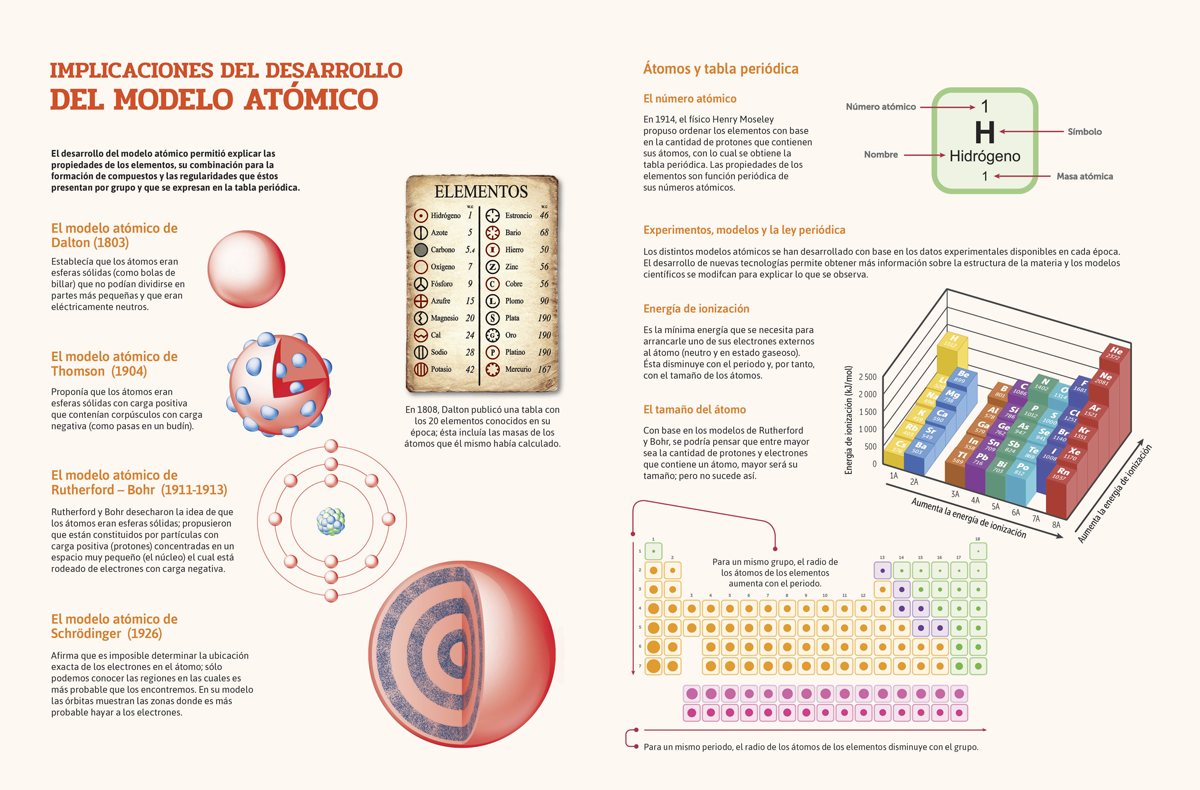
\includegraphics[width=\paperwidth]{SINQU3SB_1E16_U2_S7_114_115_INF.png}
        \label{fig:SINFI2SB_1E16_U1_S4_b_info}
        %\captionof{figure}{M\'aquinas simples.}
    \end{figure}
\end{landscape}
\newpage